\documentclass[a4paper,11pt,cours]{nsi} 
\geometry{margin=2cm}


%\setcounter{chapter}{0} % 1 de moins que le num de chapitre
%\creativecommonsfooter  %Pour marquer le doc



\begin{document}
\chapter{Premier degré}



\section{Équations du premier degré}	
\begin{definition}[s]
	\begin{enumerate}[label=\textbullet]
		\item 	On appelle \textbf{équation à une inconnue} une égalité dans laquelle figure un nombre inconnu, généralement noté $x$.
		\item 	On dit qu'un nombre est \textbf{une solution} de l'équation si et seulement si l'égalité est vérifiée lorsqu'on remplace $x$ par ce 
		nombre.
		\item 	\textbf{Résoudre} l'équation, c'est trouver \textbf{toutes les solutions} de cette équation.
	\end{enumerate}
\end{definition}



\begin{exemple}[s]
	\begin{enumerate}[label=\textbullet]
		\item Voici deux équations à une inconnue :
		
		$2x+1=-4,2x+6\qquad$ et $\qquad2\sqrt{x+1}=3x-4$\\
		\item On peut \textbf{vérifier que} 2 est \textbf{une solution} de l'équation $3x^3-1=5x^2+x+1$. En effet:
		\begin{tabbing}
			$3\times 2^3-1$	\=	$=3\times 8-1$\qquad d'une part, et d'autre part$\qquad$\= $ 5\times 2^2+2+1$\=$=5\times 4+2+1$\\
			\>	$=23$\>\>$=23$
		\end{tabbing}
	\end{enumerate}
\end{exemple}

Vérifier qu'un nombre donné est une solution d'une équation \textbf{ne suffit pas}, pour deux raisons :
\begin{enumerate}[label=\textbullet]
	\item si on ne devine aucune solution, on est « coincé ».
	\item vérifier qu'un nombre est \textbf{une} solution ne nous les fournit pas toutes.
\end{enumerate}


%\newpage

\begin {exercice}
\begin{enumerate}
	\item Vérifier que $31$ est une solution de $10x-11 = 8x +51$.
	\item Vérifier que $7$ est une solution de $\dfrac{3}{4}x+\dfrac{2}{5}=\dfrac{3}{2}x-\dfrac{97}{20}$.
	\item Vérifier que $\sqrt{2}$ est une solution de $\sqrt{2}x-\sqrt{6}=-\sqrt{3}x+2$.	
\end{enumerate}
\end {exercice}

\begin{definition}
	On appelle \textbf{équation du premier degré} toute équation de la forme
	$$ax+b = cx+d$$
	où $a$, $b$, $c$ et $d$ sont quatre nombres réels.
\end{definition}

\begin{remarque}
	$ax+b$ et $cx+d$ sont appelées des \textbf{expressions du premier degré}.
\end{remarque}

\begin{exemple}[s]
	\begin{multicols}{3}
		\begin{enumerate}[label=\textbullet]
			\item 	$34x-5=23x+50$
			\item 	$7x-2=7x+9$
			\item 	$2,4x-3=-5,7x+8$
			\item	$\displaystyle\frac{3}{4}x+1=\frac{7}{10}x-\frac{2}{7}$
			\item 	$\sqrt{2}x-2=\pi x +\sqrt{5}$
			\item	$2x-3(4x-5)=17$
		\end{enumerate}
	\end{multicols}
\end{exemple}

Pour résoudre les équations du premier degré on utilise les propriétés suivantes :

\begin{propriete}[s]
	Soient $A$, $B$ et $k$ trois nombres réels.\\
	Lorsqu'on dispose d'une égalité, on obtient une égalité équivalente en ajoutant ou en soustrayant le même nombre aux deux membres de 
	l'égalité.
	$$A=B\qquad \Longleftrightarrow\qquad A+k=B+k$$
	$$A=B\qquad \Longleftrightarrow\qquad A-k=B-k$$
	On obtient une égalité équivalente en multipliant ou en divisant les deux membres par un  même nombre non nul.\\
	Pour $k\neq 0$ :
	$$A=B\qquad \Longleftrightarrow\qquad kA=kB$$
	$$A=B\qquad \Longleftrightarrow\qquad \dfrac{A}{k}=\dfrac{B}{k}$$
\end{propriete}

Ces propriétés nous permettent d'énoncer la propriété ci dessous :

\begin{propriete}[ : Résolution des équations du premier degré ]
	
	On considère l'équation du premier degré $$ax+b=cx+d$$
	\begin{enumerate}[label=\textbullet]
		\item Si $a\neq c$ alors $\mathcal{S}=\left\{\dfrac{d-b}{a-c}\right\}$.\\
		
		\item Si $a=c$ alors ou bien $b=d$ et $\mathcal{S}=\R$, ou bien $b\neq d$ et $\mathcal{S}=\emptyset$.
	\end{enumerate}
\end{propriete}


\begin{demonstration}
			\begin{tabbing}
				$ax+b=cx+d\quad$	\=	$\Leftrightarrow\quad ax+b - cx=cx+d-cx$\\
				\>	$\Leftrightarrow\quad (a-c)x+b = d$\\[.5em]
				\>	$\Leftrightarrow\quad x=\dfrac{d-b}{a-c}\qquad$ si $a\neq c\qquad$ et $\quad\Leftrightarrow\quad b=d\quad (*)\quad$ sinon.
			\end{tabbing}
			Or
			\begin{enumerate}[label=\textbullet]
				\item 	si $b=d$ alors $(*)$ est vérifiée quelle que soit la valeur de $x$;
				\item 	sinon $b\neq d$ et quelle que soit la valeur de $x$, $(*)$ n'est pas vérifiée.
			\end{enumerate}
	%\petitscarreaux{16.5}{10}
\end{demonstration}	

\begin{remarque}
	En pratique, on n'utilise pas cette propriété, on « isole les $x$ » dans un des membres de l'égalité, les constantes de l'autre, puis on 
	divise les deux membres de l'équation par le coefficient de $x$ (pour peu qu'il soit non nul).
\end{remarque}


\begin {exercice}
Résoudre les équations suivantes :
\begin{multicols}{2}
	\begin{enumerate}
		\item 	$34x-5=23x+50$
		\item 	$3x+1 = 3x -7$
		\item 	$2,4x-3=-5,7x+8$
		\item	$\displaystyle\frac{3}{4}x+1=\frac{7}{10}x-\frac{2}{7}$
		%\item	$\displaystyle\frac{1}{2}x+\dfrac{1}{3}=\frac{1}{4}x+\frac{1}{5}$
		\item 	$\sqrt{2}x-2=\pi x +\sqrt{5}$
		\item	$2x-3(4x-5)=17$
	\end{enumerate}
\end{multicols}
\end {exercice}

\section{\'Equations se ramenant à des équations du premier degré}

Grâce à la propriété suivante, on peut ramener la résolution de certaines équations de degré supérieur à 1 à une résolution d'équation de degré 1.

\begin{propriete}[]
	Un produit de facteurs est nul si, et seulement si, au moins l'un de ses facteurs est nul.
\end{propriete}

Cette propriété permet de résoudre des équations \textbf{produit-nul} ou des équation s'y ramenant.

\begin{exemple}[s]
	\begin{itemize}
		\item 	$(3x-5)(4x+8)=0 \quad$ est une équation produit-nul.
		\item	$x^2+3x-5=x^2-7x-4 \quad$ est une équation du second degré.\\
		Après soustraction de $x^2$ à chacun de ses membres, on obtient l'équation équivalente \\$\quad 3x-5=-7x-4 \quad$ qui est une équation du premier degré.
	\end{itemize}
\end{exemple}

\begin{exercice}[]
	Résoudre les équations suivantes :
	\begin{multicols}{2}
		\begin{enumerate}
			\item 	$(3x-5)(4x+8)=0$
			\item 	$x^2+3x-5=x^2-7x-4$
			\item	$(x-5)^2=(x+4)^2$
			\item	$(2x-1)(3x+2)+(2x-1)(7-x)=0$
			\item	$(4x-1)(x-7)-(x-7)^2=0$\\
				
		\end{enumerate}
	\end{multicols}
\end{exercice}

\section{Inéquations du premier degré}

On retrouve ici beaucoup de notions similaires à celles de la partie précédente.

\begin{definition}[s]
	\begin{enumerate}[label=\textbullet]
		\item 	On appelle \textbf{inéquation à une inconnue} une inégalité dans laquelle figure un nombre inconnu, généralement noté $x$.
		\item 	On dit qu'un nombre est \textbf{une solution} de l'inéquation si et seulement si l'inégalité est vérifiée lorsqu'on remplace $x$ 
		par ce nombre.
		\item 	\textbf{Résoudre} l'inéquation, c'est trouver \emph{toutes les solutions} de cette équation.
	\end{enumerate}
\end{definition}

\begin{exemple}[s]
	\begin{enumerate}[label=\textbullet]
		\item Voici deux inéquations à une inconnue :
		
		$x-1<-5x+6\qquad$ et $\qquad2\sqrt{x+2}\geqslant 3x+4$
		\item On peut \emph{vérifier que} -2 est \emph{une solution} de l'inéquation $3x^2-1<2x^2+x+10$. En effet:
		\begin{tabbing}
			$3\times (-2)^2-1$	\=	$=3\times 4-1$\qquad et d'autre part$\qquad$\= $ 2\times(-2)^2+(-2)+10$\=$=8-2+10$\\
			\>	$=11$\>\>$=16$
		\end{tabbing}
	\end{enumerate}
\end{exemple}

Pour résoudre les inéquations du premier degré on utilise les propriétés suivantes :

\begin{propriete}[s]\textbf{\boldmath Valables avec <, >, $\geqslant$, $\leqslant$ :}\\[0.5em]
	Soient $A$, $B$ et $k$ trois nombres réels.\\
	Lorsqu'on dispose d'une inégalité, on obtient une inégalité équivalente en ajoutant ou en soustrayant le même nombre aux deux membres de 
	l'égalité.
	$$A<B\qquad \Longleftrightarrow\qquad A+k<B+k$$
	$$A<B\qquad \Longleftrightarrow\qquad A-k<B-k$$
	On obtient une inégalité équivalente en multipliant ou en divisant les deux membres par un  même nombre \textbf{strictement positif}.\\
	Pour $k>0$ :
	$$A<B\qquad \Longleftrightarrow\qquad kA<kB$$
	$$A<B\qquad \Longleftrightarrow\qquad \dfrac{A}{k}<\dfrac{B}{k}$$
	
	Lorsqu'on multiplie ou qu'on divise les deux membres par un  même nombre \textbf{strictement négatif}, on obtient une inégalité équivalent 
	\textbf{en « retournant » le symbole de comparaison}. \\
	Pour $k<0$ :
	$$A<B\qquad \Longleftrightarrow\qquad kA>kB$$
	$$A<B\qquad \Longleftrightarrow\qquad \dfrac{A}{k}>\dfrac{B}{k}$$
\end{propriete}

\begin{methode} \textbf{\boldmath Résoudre $4x-5\leqslant 7x+40$ :}
	\begin{tabbing}
		$4x-5\leqslant 7x+40\quad$	\=	$\Leftrightarrow\quad 4x-5 +5\leqslant 7x+40 +5$\\
		\>	$\Leftrightarrow\quad 4x\leqslant 7x+45$\\
		\>	$\Leftrightarrow\quad 4x-7x\leqslant 7x+45-7x$\\
		\>	$\Leftrightarrow\quad 4x-7x\leqslant 7x+45-7x$\\
		\>	$\Leftrightarrow\quad -3x\leqslant 45\qquad$ on va diviser par un nombre négatif.\\[.5em]
		\>	$\Leftrightarrow\quad x\geqslant\dfrac{45}{-3}$\\[.5em]
		\>	$\Leftrightarrow\quad x\geqslant-15\quad$ ainsi $\quad\mathcal{S}=\fii{-15}$
	\end{tabbing}
	\begin{center}
		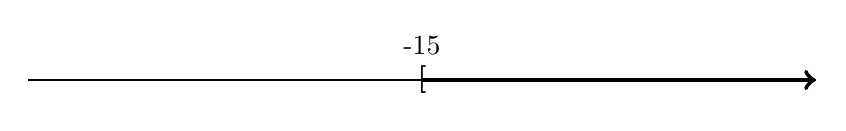
\begin{tikzpicture}
			\draw (-20,0)--(-10,0);
			\draw[ultra thick,->] (-15,0)node{\textbf{[}} node[above=.5em] {-15}--(-10,0);
		\end{tikzpicture}\\
		\emph{Schéma de l'ensemble des solutions}\\
	\end{center}
\end{methode}


\begin {exercice}
Résoudre les inéquations suivantes et faire un schéma de l'ensemble des solutions.
\begin{multicols}{2}
	\begin{enumerate}
		\item 	$2x-5<7x-35$
		\item 	$3x+1 > -8x -7$
		\item 	$-1,2x-8,1>3,2x+5,7$
		\item 	$1,4x-3\geqslant-5,7x-18$
		\item	$\displaystyle\frac{2}{5}x+1\leqslant\frac{7}{10}x+\frac{2}{3}$
		\item	$\displaystyle\frac{3}{2}x+\dfrac{2}{3}>-\frac{1}{4}x+\frac{1}{5}$
	\end{enumerate}
\end{multicols}
\end {exercice}

\section{Signe d'une expression du premier degré et applications}

\begin{propriete}
	Soit $ax+b$ une expression du premier degré, où $a$ et $b$ sont deux réels et $a\neq 0$. On a le tableau de signe suivant :
	
	\textbf{\boldmath si $a>0$ :}
	\begin{center}
		\begin{tikzpicture}
			\tkzTabInit[color,lgt=3.5,espcl=3]
			{$x$ /1 ,signe de $ax+b$ /1}
			{$-\infty$, $-\dfrac{b}{a}$ ,$+\infty$ }
			\tkzTabLine{,- , z, +,}
		\end{tikzpicture}
	\end{center}
	
	\textbf{\boldmath si $a<0$ :}
	\begin{center}
		\begin{tikzpicture}
			\tkzTabInit[color,lgt=3.5,espcl=3]
			{$x$ /1 ,signe de $ax+b$ /1}
			{$-\infty$, $-\dfrac{b}{a}$ ,$+\infty$ }
			\tkzTabLine{,+ , z, -,}
		\end{tikzpicture}
	\end{center}
\end{propriete}

\begin{demonstration}
			\begin{tabbing}
				$ax+b>0\quad$	\=	$\Leftrightarrow\quad ax>-b$\\
				\>	$\Leftrightarrow\quad x>-\dfrac{b}{a}\qquad$ si $a>0\qquad$ ou $\qquad x<-\dfrac{b}{a}\qquad$ si $a<0$
			\end{tabbing}
\end{demonstration}

%\newpage

\begin {exercice}
Donner le tableau de signes des expressions suivantes :
\begin{multicols}{2}
	\begin{enumerate}
		\item 	$3x+2$
		\item 	$-4x-9$
		\item 	$\dfrac{3}{5}x-\dfrac{2}{7}$
		\item 	$\sqrt{3}x-3$
		\item 	$(2x-1)(-3x+2)$
		\item	$\dfrac{5x-2}{-7x-8}$
	\end{enumerate}
\end{multicols}\ \\[-2em]
Pour les deux dernières on étudiera le signe de chaque expression du premier degré puis on utilisera la règle des signes.
\end {exercice}

\section{\'Equations de droites}
Le plan est muni d'un repère $\rep$.
\begin{center}
	\def\xmin{-1} \def\ymin{-1}\def\xmax{7}\def\ymax{5}
	\def\F{-2/3*(\x-1)+3}
	\begin{tikzpicture}[scale=1.3]
		\clip (\xmin,\ymin) rectangle (\xmax,\ymax);
		\draw[fill = white] (\xmin,\ymin) rectangle (\xmax,\ymax);
		\reperevl{\xmin}{\ymin}{\xmax}{\ymax}
		\draw[very thick,domain=\xmin:\xmax,smooth,variable=\x] plot ({\x},{\F});
		\draw (0,11/3)\ball node[above right]{$(0,p)$};
		\draw (1,3)\ball node [below] {A} (4,1)\ball node [below] {B}(2,7/3)\ball;
		\draw[thick,->] (1,3)-- node[midway,above] {\tiny$x$ augmente de 1}(2,3);
		\draw[thick,->,dashed] (1,3)-- node[midway,above=2em ] {\tiny $x$ augmente de 3}(4,3);
		\draw[thick,->] (2,3) -- node [midway,right]{\tiny $y$ diminue de $\dfrac{2}{3}$} ( 2,7/3);
		\draw[thick,->,dashed] (4,3) -- node [midway,right]{\tiny $y$ diminue de $2$} ( 4,1);
		\draw (1,3)--node[sloped,midway,below]{coefficient directeur : $-\dfrac{2}{3}$}(4,1);
	\end{tikzpicture}
\end{center}

\begin{propriete}
	Soit $(d)$ une droite d'équation $y=mx+p$ dans le repère $\rep$.
	\begin{enumerate}[label=\textbullet]
		\item 	$p$ s'appelle \textbf{l'ordonnée à l'origine} : $(d)$ passe par le point de coordonnées $(0\ ;p)$.
		\item 	$m$ s'appelle le \textbf{coefficient directeur} : dès que $A$ et $B$ sont deux points distincts de $(d)$ alors $$\boldmath 
		m=\dfrac{y_B-y_A}{x_B-x_A}$$
	\end{enumerate}
\end{propriete}
\begin {exercice}
Sans justifier, lire les équations des droites $(d_1)$ à $(d_5)$ du graphique suivant :
\def\xmin{-11}	\def\xmax{11}	\def\ymin{-9}	\def\ymax{9}
\begin{center}
	\begin{tikzpicture}[scale = 16/22]
		\draw[fill=white](\xmin,\ymin) rectangle (\xmax,\ymax);
		\reperevl{\xmin}{\ymin}{\xmax}{\ymax}
		\clip (\xmin,\ymin) rectangle (\xmax,\ymax);
		\draw[domain=\xmin:\xmax,samples=2,variable=\x] plot ({\x},{0.75*\x-6});
		\draw[domain=\xmin:\xmax,samples=2,variable=\x] plot ({\x},{3*\x-5});
		\draw[domain=\xmin:\xmax,samples=2,variable=\x] plot ({\x},{-4*\x+7});
		\draw[domain=\xmin:\xmax,samples=2,variable=\x] plot ({\x},{-0.25*\x+2});
		\draw[domain=\xmin:\xmax,samples=2,variable=\x] plot ({\x},{0.1*\x});
		\draw[domain=\xmin:\xmax,samples=2,variable=\x] plot ({\x},{0.5*\x-4});
		\draw[domain=\xmin:\xmax,samples=2,variable=\x] plot ({\x},{-\x+15});
		\draw[domain=\xmin:\xmax,samples=2,variable=\x] plot ({\x},{-3/7*\x+9/7});
		
		\node[rotate=5] () 	at 	(-10.5,-.7){$(d_1)$};
		\node[rotate=-13]() at 	(-10.5,5){$(d_2)$};
		\node[rotate=40]() 	at	(-4,-8.5){$(d_3)$}		;
		\node[rotate=70]()	at 	(-1.5,-8.5){$(d_4)$};	
		\node[rotate=-70]()	at	(-1,8.5){$(d_5)$}	;
		\draw (-10,-1)\ball  node[below]{A} (0,2) \ball node[below left]{C} (-4,3) \ball node[below left]{D} (0,7)\ball node[right]{E} 
		(1,3)\ball node[right]{F} (0,-5)\ball node[above left]{G}(1,-2)\ball node[above left]{H}(0,-6)\ball node[below 
		right]{K}(4,-3)\ball node[below right]{L}(-6,-7)\ball node[below right]{M}(-2,-5)\ball node[below right]{N}(9,6)\ball node[above 
		right]{R}(7,8)\ball node[above right]{S}(10,-3)\ball node[below left]{U};
	\end{tikzpicture}
\end{center}
\end {exercice}

\begin{methode}\textbf{Déterminer par le calcul l'équation réduite d'une droite passant par 2 points donnés :}\\[.5em]
	Déterminons l'équation réduite de $(MN)$ : $x_M\neq x_N$ donc cette droite n'est pas parallèle à l'axe des ordonnées, elle admet donc une 
	unique équation du type $y=mx+p$.
	%		\breakbox
	\begin{multicols}{2}
		\textbf{1. Déterminons m :}
		\begin{tabbing}
			$m$	\= 	$=\dfrac{y_N-y_M}{x_N-x_M}$	\\[0.4em]	
			\>	$=\dfrac{-5-(-7)}{-2-(-4)}$	\\[0.4em]
			\>	$=\dfrac{2}{4}$	\\[0.4em]
			\>	$=\dfrac{1}{2}$
		\end{tabbing}
		\columnbreak
		\textbf{2. Déterminons p:}\\
		Puisque $(MN)\ :\ y=\dfrac{1}{2}x+p$ et que $\pc{M}{-6}{-7}\in(MN)$ alors
		\begin{tabbing}
			$y_M=\dfrac{1}{2}x+p\quad$	\=	$\Leftrightarrow\quad -7=\dfrac{1}{2}\times(-6)+p$\\[0.3em]
			\>	$\Leftrightarrow\quad -7=-3+p$\\
			\>	$\Leftrightarrow\quad p=-4$
		\end{tabbing}
	\end{multicols}
	\begin{center}
		Ainsi $(MN)\ :\ y=\dfrac{1}{2}x-4$.
	\end{center}
\end{methode}

%\newpage

\begin {exercice}
Déterminer les équations réduites des droites $(SR)$ et $(DU)$ du graphique précédent.\\

Déterminer et tracer sur le graphique précédent l'équation réduite de la droite passant par $\pc{B}{300}{-95}$ et $\pc{T}{-111}{42}$.
\end {exercice}

\section{Fonctions affines}
\begin{definition}[]
	Une fonction $f$ est dite \textbf{affine} si :
	\begin{enumerate}[label=\textbullet]
		\item 	elle est \textbf{définie sur \R} ;
		\item 	on peut écrire : pour tout $x \in \R, \quad f(x)=mx+p \quad$ où $m$ et $p$ sont deux nombres réels.
	\end{enumerate}
\end{definition}

\begin{exemple}[s]
	\begin{enumerate}[label=\textbullet]
		\item 	$f$ définie sur $\R$ par $f(x)=3x+2$ est affine ($m=3$ et $p=2$).
		\item 	$g$ définie sur $\R$ par $g(x)=-\dfrac{7}{3}x+\dfrac{2}{5}$ l'est également ($m=-\dfrac{7}{3}$ et $p=\dfrac{2}{5}$).
		\item 	En dépit des apparences, $h$ définie sur $\R$ par $h(x)=(x+2)^2-(x-1)^2$ est une fonction affine car on peut écrire pour tout $x\in\R$
		\begin{tabbing}
			$h(x)$	\=	$=x^2+4x+4-(x^2-2x+1)$\\
			\>	$=x^2+4x+4-x^2+2x-1\qquad$\= \\
			\>	$=6x+3$ \>et donc $m=6$ et $p=3$.
		\end{tabbing}
		
	\end{enumerate}
\end{exemple}

\begin{remarque}[s]
	
	\begin{enumerate}[label=\textbullet]
		\item 	{\boldmath\textbf{Si $p=0$} alors $f$ est définie sur $\R$ par $f(x)=mx$ : c'est une \textbf{fonction linéaire}}.
		\begin{center}
			\def\xmin{-3} \def\ymin{-3}\def\xmax{3}\def\ymax{3}
			\def\F{0.5*\x}
			\begin{tikzpicture}[scale=.5]
				\clip (\xmin,\ymin) rectangle (\xmax,\ymax);
				\draw[fill = white] (\xmin,\ymin) rectangle (\xmax,\ymax);
				\repereal{\xmin}{\ymin}{\xmax}{\ymax}
				\draw[UGLiRed,thick,domain=\xmin:\xmax,smooth,variable=\x] plot ({\x},{\F});		
			\end{tikzpicture}\\
			\emph{\footnotesize courbe représentative de $f$ définie sur $\R$ par $f(x)=\dfrac{1}{2}x$}
		\end{center}
		\item 	{\boldmath\textbf{Si $m=0$} alors $f$ est définie sur $\R$ par $f(x)=p$ : c'est une \textbf{fonction constante}}.
		\begin{center}
			\def\xmin{-3} \def\ymin{-3}\def\xmax{3}\def\ymax{3}
			\def\F{2}
			\begin{tikzpicture}[scale=.5]
				\clip (\xmin,\ymin) rectangle (\xmax,\ymax);
				\draw[fill = white] (\xmin,\ymin) rectangle (\xmax,\ymax);
				\repereal{\xmin}{\ymin}{\xmax}{\ymax}
				\draw[UGLiRed,thick,domain=\xmin:\xmax,smooth,variable=\x] plot ({\x},{\F});		
			\end{tikzpicture}\\
			\emph{\footnotesize courbe représentative de $f$ définie sur $\R$ par $f(x)=2$}
		\end{center}
	\end{enumerate}
	
\end{remarque}

\begin{propriete}[ et définition]
	Soit $f$ une fonction affine définie sur $\R$ par $f(x)=mx+p$.
	
	\begin{enumerate}[label=\textbullet]
		\item 	$p$ est {\boldmath\textbf{l'image de 0}} par $f$, donc $\courbe{f}$ passe par le point $\pc{P}{0}{p}$.
		\item 	{\boldmath\textbf{$\courbe{f}$ est une droite.}}

	\def\xmin{-1} \def\ymin{-1}\def\xmax{7}\def\ymax{5}
	\def\F{-.5*\x+3}
	\begin{center}\begin{tikzpicture}
			\clip (\xmin,\ymin) rectangle (\xmax,\ymax);
			\draw[fill = white] (\xmin,\ymin) rectangle (\xmax,\ymax);
			\reperev{\xmin}{\ymin}{\xmax}{\ymax}
			\draw (0,3)\ball node[above right]{$\pc{P}{0}{p}$};
			\draw[color=UGLiRed,thick,domain=\xmin:\xmax,smooth,variable=\x] plot ({\x},{\F});	
			\draw[color =UGLiRed] (4,1) node [above right]{$\courbe{f}$};	
	\end{tikzpicture}\end{center}
	
		\item	Le nombre $m$ s'appelle le {\boldmath\textbf{taux d'accroissement de $f$}}.\\
		Pour tous nombres \textbf{distincts} $x_1$ et $x_2$ on a {\boldmath\textbf{$$m = \dfrac{f(x_2)-f(x_1)}{x_2-x_2}$$}}
	\end{enumerate}
	\def\xmin{-.5} \def\ymin{-.5}\def\xmax{4}\def\ymax{2}
	\def\F{-.5*\x+1.5}
	\begin{center}\begin{tikzpicture}[scale = 2.5]
			\clip (\xmin,\ymin) rectangle (\xmax,\ymax);
			\draw[fill = white] (\xmin,\ymin) rectangle (\xmax,\ymax);
			\reperev{\xmin}{\ymin}{\xmax}{\ymax}
			\pointc{1}{1}{$x_1$}{$f(x_1)$}{}
			\pointc{2}{.5}{$x_2$}{$f(x_2)$}{}	
			\draw[color=UGLiRed,thick,domain=\xmin:\xmax,smooth,variable=\x] plot ({\x},{\F});
			\draw[->,very thick,color = UGLiGreen,dashed] (1,1)-- node[midway,above]{variation : $x_2-x_1$}(2,1);
			\draw[->,very thick,color = UGLiGreen,dashed](2,1) -- node[midway,right]{variation :
				$f(x_2)-f(x_1)$}(2,.5);
			\draw[color =UGLiRed] (.5,1.25) node [above right]{$\courbe{f}$};	
	\end{tikzpicture}\end{center}
\end{propriete}
\begin{demonstration}
	\begin{enumerate}[label=\textbullet]
		\item 	\begin{tabbing}
			$f(0)$ 	\=  $= m\times 0+p $\\
			\>  $= p$ \hspace*{2cm} donc $P(0;p) \in \mathcal{C}_f$.
		\end{tabbing}
		\item 	$\mathcal{C}_f : y=mx+p$\\
			On reconnait l'équation d'une droite de coefficient directeur $m$ et d'ordonnée à l'origine $p$.
		\item	Soient $\quad M_1(x_1;f(x_1))\quad$ et $\quad M_2(x_2;f(x_2))$.
		\begin{tabbing}
			$M_1$ et $M_2$ appartiennent à $\mathcal{C}_f$, donc $\quad m $ 	\=  $=\dfrac{y_{M_2}-y_{M_1}}{x_{M_2}-x_{M_1}} $\\[.7em]
			\>  $= \dfrac{f(x_2)-f(x_1)}{x_2-x_1}$
		\end{tabbing}
		
	\end{enumerate}
	%\petitscarreaux{16.5}{12}
\end{demonstration}

\begin{methode}[ : déterminer l'expression algébrique d'une fonction affine]\ \\[-1.5em]
	
	$f$ est une fonction affine. $f(-3)=2$ et $f(2)=-4$. Déterminons l'expression algébrique de $f$.
	\begin{enumerate}[label=\textbullet]
		\item 	Puisque $f$ est affine, pour tout $x\in\R$ on a $f(x)=mx+p$.
		\begin{multicols}{2}
			\item 	\textbf{Déterminons m :}
			\begin{tabbing}
				$m$	\=	$=\dfrac{f(2)-f(-3)}{2-(-3)}$\\[.5em]
				\>	$=\dfrac{-4-2}{2+3}$\\[.5em]
				\> 	$=\dfrac{-6}{5}$
			\end{tabbing}
			Ainsi pour tout $x\in\R$ on a $f(x)=-\dfrac{6}{5}x+p$.\\
			\vspace{.5cm}
			\item 	\textbf{Déterminons p :}\\
			Puisque $f(-3)=2$ on peut écrire :
			\begin{tabbing}
				$\underbrace{-\dfrac{6}{5}\times (-3)+p}_{f(-3)}=2$\quad	\=	$\Leftrightarrow\quad \dfrac{18}{5}+p=2$\\
				\>	$\Leftrightarrow\quad p=2-\dfrac{18}{5}$\\[.5em]
				\>	$\Leftrightarrow\quad p=\dfrac{10}{5}-\dfrac{18}{5}$\\[.5em]
				\>	$\Leftrightarrow\quad p=-\dfrac{8}{5}$													
			\end{tabbing}
		\end{multicols}
		
		\item 	Ainsi, {\boldmath\textbf{pour tout $x\in\R$, on a $f(x)=-\dfrac{6}{5}x-\dfrac{8}{5}$}}.
	\end{enumerate}
	\begin{center}
		\def\xmin{-4} \def\ymin{-5}\def\xmax{3}\def\ymax{3}
		\def\F{-1.2*\x-1.6}
		\begin{tikzpicture}[scale=.65]
			\clip (\xmin,\ymin) rectangle (\xmax,\ymax);
			\draw[fill = white] (\xmin,\ymin) rectangle (\xmax,\ymax);
			\reperevl{\xmin}{\ymin}{\xmax}{\ymax}
			\pointcx{2}{-4}{2}{-4}{}
			\pointcx{-3}{2}{-3}{2}{}
			\draw[UGLiRed,thick,domain=\xmin:\xmax,smooth,variable=\x] plot ({\x},{\F});
			\draw (-3,2)\ball node[UGLiRed,above right]{$\courbe{f}$}  (2,-4)\ball;		
		\end{tikzpicture}
	\end{center}
\end{methode}

\begin{remarque}[]
	Pour déterminer $p$ on aurait tout aussi bien pu écrire que $f(2)=-4$, on aurait également abouti à $p=-\dfrac{8}{5}$.
\end{remarque}

\begin{propriete}[ : signe d'une fonction affine]
	Soit $f$ une fonction affine définie sur $\R$ par $f(x)=mx+p$.\\
	Si $m\neq 0$ alors $f$ admet le tableau de signe suivant :
	\begin{enumerate}[label=\textbullet]
		\item 	\textbf{\boldmath Si $m>0$ :}\begin{center}
			\begin{tikzpicture}
				\tkzTabInit[color,lgt=3.5,espcl=3]
				{$x$ /1 ,$f(x)$ /1}
				{$-\infty$, $-\dfrac{p}{m}$ ,$+\infty$ }
				\tkzTabLine{,- , z, +,}
			\end{tikzpicture}
		\end{center}
		
		\item 	\textbf{\boldmath Si $m<0$ :}\begin{center}
			\begin{tikzpicture}
				\tkzTabInit[color,lgt=3.5,espcl=3]
				{$x$ /1 ,$f(x)$ /1}
				{$-\infty$, $-\dfrac{p}{m}$ ,$+\infty$ }
				\tkzTabLine{,+ , z, -,}
			\end{tikzpicture}
		\end{center}
	\end{enumerate}
\end{propriete}
\begin{demonstration}
	Par \textbf{disjonction de cas} :
	\begin{multicols}{2}
		\begin{enumerate}[label=\textbullet]
			\item 	Si $m>0$ :
			\begin{tabbing}
				$f(x)>0 \quad$		\=	$\Leftrightarrow\quad mx+p>0$\\
				\>	$\Leftrightarrow\quad mx>-p$\\
				\>	$\Leftrightarrow\quad x>-\dfrac{p}{m}$
			\end{tabbing}
			\item 	 	Si $m<0$ :
			\begin{tabbing}
				$f(x)>0 \quad$		\=	$\Leftrightarrow\quad mx+p>0$\\
				\>	$\Leftrightarrow\quad mx>-p$\\
				\>	$\Leftrightarrow\quad m<-\dfrac{p}{m}$
			\end{tabbing}
		\end{enumerate}
	\end{multicols}
	
	%\petitscarreaux{16.5}{9}
\end{demonstration}

%\newpage



\section{Systèmes linéaires d'équations}
\begin{definition}[s]
	\begin{enumerate}[label=\textbullet]
		\item 	Un \textbf{système linéaire de deux équations à deux inconnues} $x$ et $y$ est un système qui peut s'écrire sous la forme :
		$$\left\{
		\begin{array}{cll}
			\ ax+by&=&c \\
			\ a'x+b'y&=&c' \\
		\end{array} \right. \qquad \text{où }a,b,c,a',b'\text{ et }c'\text{sont des réels fixés.} $$
		\item 	Une solution de ce système est un \textbf{couple} $(x\ ;y)$ de deux nombres réels tel que $x$ et $y$ vérifient simultanément les deux équations.	
	\end{enumerate}
\end{definition}

\begin{exemple}[s]
	\begin{enumerate}[label=\textbullet]
		\item 	$\left\{
		\begin{array}{cll}
			\ x+5y&=&19 \\
			\ -2x+y&=&-5 \\
		\end{array} \right.\quad$ est un système linéaire de deux équations à deux inconnues.
		\item 	Le couple $(4\ ;3)$ est solution de ce système car il vérifie les deux équations en même temps.\\
		En effet : $\quad 4+5\times3=19 \quad$ et $\quad-2\times4+3=-5$.
		\item	Le couple $(9\ ;2)$ n'est pas solution de ce système car il vérifie que la première équation mais pas la seconde.\\
		En effet : $\quad 9+5\times2=19 \quad$ et $\quad-2\times9+=-16\neq-5$.
	\end{enumerate}
\end{exemple}

\begin{exercice}[ ]
	\begin{enumerate}
		\item 	Le couple $(4\ ;-2)$ est-il solution du système $\left\{
		\begin{array}{l}
			\ 2x+y=6 \\
			\ y=x-6 \\
		\end{array} \right.$ ?
		\item 	Le couple $(2\ ;1)$ est -il solution du système $\left\{
		\begin{array}{l}
			\ 2x+3y=8 \\
			\ 3x-2y=-1 \\
		\end{array} \right.$ ?
	\end{enumerate}
\end{exercice}

\begin{propriete}[ ]
	On obtient un système équivalent à un système donné en:
	\begin{enumerate}[label=\textbullet]
		\item 	remplaçant une équation par un équation équivalente ;
		\item 	substituant une expression par une expression équivalente ;
		\item	remplaçant une des équations par la somme ou la différence membre à membre des équations.	
	\end{enumerate}
\end{propriete}

\begin{methode}[ ]\textbf{Résoudre graphiquement un système linéaire }\\
	On cherche à résoudre le système linéaire 
	$\left\{
	\begin{array}{cll}
		\ -2x+y&=&4 \\
		\ x+y&=&1 \\
	\end{array} \right.$\\
	On transforme ce système en un système équivalent : $\left\{
	\begin{array}{cll}
		\ y&=&2x+4 \\
		\ y&=&-x+1 \\
	\end{array} \right.$\\
	$y=2x+4$ et $y=-x+1$ sont les équations de deux droites $(d_1)$ et $(d_2)$.\\
	On représente graphiquement ces droites. Les solutions de ce système sont les coordonnées des points appartenant aux deux droites.
	\def\xmin{-4}	\def\xmax{4}	\def\ymin{-4}	\def\ymax{4}
	\begin{center}
		\begin{tikzpicture}[scale = 16/22]
			\draw[fill=white](\xmin,\ymin) rectangle (\xmax,\ymax);
			\reperevl{\xmin}{\ymin}{\xmax}{\ymax}
			\clip (\xmin,\ymin) rectangle (\xmax,\ymax);
			\draw[domain=\xmin:\xmax,samples=2,variable=\x] plot ({\x},{2*\x+4});
			\draw[domain=\xmin:\xmax,samples=2,variable=\x] plot ({\x},{-1*\x+1});
			\node[rotate=60] () 	at 	(-3,-3){$(d_1)$};
			\node[rotate=-45]() at 	(-3,3){$(d_2)$};
			\draw (-1,2)\ball  node[above]{P};
		\end{tikzpicture}
	\end{center}
	Les droites $(d_1)$ et $(d_2)$ sont sécantes en $P(-1\ ;2)$.\\
	La solution du système est donc le couple $(-1\ ;2)$.
\end{methode}

\begin{remarque}[s]
	\begin{enumerate}[label=\textbullet]
		\item 	Cette méthode de résolution est assez limitée. Parfois, les coordonnées du point d'intersection ne sont pas évidentes à lire de manière exacte. On préférera alors des méthodes calculatoires.
		\item 	Si les deux droites sont sécantes, alors le système a un unique couple solution.\\[0.5em]
		Si les deux droites sont parallèles, alors le système a :
		\begin{itemize}
			\item 	soit aucune solution dans le cas où les droites sont strictement parallèles ;
			\item 	soit une infinité de solutions dans le cas où les droites sont confondues.
		\end{itemize}	
	\end{enumerate}
\end{remarque}



\begin{exercice}[ ]
	
	\begin{multicols}{3}
		Résoudre graphiquement les systèmes suivants :\\
		\vspace{1cm}
		\begin{enumerate}
			\item 	$\left\{
			\begin{array}{l}
				\ y=2x+1 \\
				\ y=-3x+6 \\
			\end{array} \right.$
			\item 	$\left\{
			\begin{array}{l}
				\ y=5x+6 \\
				\ x=-2 \\
			\end{array} \right.$
			\item 	$\left\{
			\begin{array}{l}
				\ y=x-3 \\
				\ 2x+y=3 \\
			\end{array} \right.$
			\item 	$\left\{
			\begin{array}{l}
				\ x-2y=-7 \\
				\ 2x-y=-5 \\
			\end{array} \right.$	
		\end{enumerate}
	\end{multicols}
\end{exercice}

\begin{methode}[ ]\textbf{Résolution par substitution}
	\begin{enumerate}[label=\textbullet]
		\item 	\textbf{\'Etape 1 :} on isole une inconnue dans une des équations.
		\item 	\textbf{\'Etape 2 :} on la remplace dans l'autre équation par l'expression trouvée.
		\item	\textbf{\'Etape 3 :} on résout l'équation à une inconnue obtenue.
		\item	\textbf{\'Etape 4 :} on en déduit l'autre inconnue puis le couple solution.	
	\end{enumerate}
	Résolvons par substitution le système $\quad (S):\left\{
	\begin{array}{cll}
		\ 3x+y&=&14 \\
		\ 7x-4y&=&1 \\
	\end{array} \right.$\\
	
	\vspace{0.3cm}
	\begin{tabular}{p{9cm}p{7cm}}
		
		\textbf{\'Etape 1 :} on isole $y$ dans la première équation. & $(S) \Leftrightarrow \left\{
		\begin{array}{l}
			\ y=-3x+14 \\
			\ 7x-4y=1 \\
		\end{array} \right.$\\
		
		\textbf{\'Etape 2 :} on remplace $y$ par l'expression trouvée dans la deuxième équation &  $(S) \Leftrightarrow \left\{
		\begin{array}{l}
			\ y=-3x+14 \\
			\ 7x-4(-3x+14)=1 \\
		\end{array} \right.$\\
		& $(S) \Leftrightarrow \left\{
		\begin{array}{l}
			\ y=-3x+14 \\
			\ 19x-56=1 \\
		\end{array} \right.$\\
		
		\textbf{\'Etape 3 :} on résout l'équation ainsi obtenue qui ne comporte plus qu'une seule inconnue $x$ & $(S) \Leftrightarrow \left\{
		\begin{array}{l}
			\ y=-3x+14 \\
			\ x=\dfrac{57}{19}=3 \\
		\end{array} \right.$\\
		
		\textbf{\'Etape 4 :} on	peut alors calculer l'autre inconnue et obtenir le couple solution. & $(S) \Leftrightarrow \left\{
		\begin{array}{l}
			\ y=-3\times3+14 \\
			\ x=3 \\
		\end{array} \right.$\\
		& $(S) \Leftrightarrow \left\{
		\begin{array}{l}
			\ y=5 \\
			\ x=3 \\
		\end{array} \right.$\\
	\end{tabular}
	Le couple $(3\ ;5)$ est la solution de ce système.
\end{methode}

\begin{remarque}[s]
	La méthode de résolution par substitution est efficace lorsqu'il est facile d'exprimer une inconnue en fonction de l'autre.\\
	Dans l'exemple précédent on a choisit d'écrire $\quad 3x+y=14 \Leftrightarrow y=-3x+14$.\\
	On aurait pû écrire  $\quad 3x+y=14 \Leftrightarrow x=-\dfrac{1}{3}y+\dfrac{14}{3}\quad$ mais cette expression est plus difficile à utiliser ensuite (du fait des fractions).
\end{remarque}

\begin{exercice}[ ]
	
	\begin{multicols}{3}
		Résoudre chacun des systèmes par substitution.\\
		\vspace{1cm}
		\begin{enumerate}
			\item 		$\left\{
			\begin{array}{l}
				\ x+3y=8 \\
				\ 2x-5y=-17\\
			\end{array} \right.$
			\item 		$\left\{
			\begin{array}{l}
				\ 2x+y=4 \\
				\ 5x+3y=9 \\
			\end{array} \right.$	
			\item 		$\left\{
			\begin{array}{l}
				\ 4x-3y=-13 \\
				\ 4x-y=1 \\
			\end{array} \right.$
			\item 		$\left\{
			\begin{array}{l}
				\ 8x+3y=-4 \\
				\ x+5y=1 \\
			\end{array} \right.$
		\end{enumerate}
	\end{multicols}
\end{exercice}

\begin{methode}[ ]\textbf{Résolution par combinaisons linéaires}
	\begin{enumerate}[label=\textbullet]
		\item 	\textbf{\'Etape 1 :} on remplace les équations par des équations équivalentes dans lesquelles une inconnue a le même coefficient (ou des coefficients opposés).
		\item 	\textbf{\'Etape 2 :} on la remplace une équation par la somme ou ka différence membre à membre des deux équations.
		\item	\textbf{\'Etape 3 :} on résout l'équation à une inconnue obtenue.
		\item	\textbf{\'Etape 4 :} on en déduit l'autre inconnue puis le couple solution.	
	\end{enumerate}
	Résolvons par combinaisons linéaires le système $\quad (S):\left\{
	\begin{array}{cll}
		\ 3x+y&=&14 \\
		\ 7x-4y&=&1 \\
	\end{array} \right.$\\
	
	\begin{tabular}{p{8cm}p{8cm}}
		\textbf{\'Etape 1 :} on multiplie par 4 chaque membre de la première équation pour obtenir $4y$ dans les deux équations. & $(S) \Leftrightarrow \left\{
		\begin{array}{cll}
			\ 4(3x+y)&=&4\times14 \\
			\ 7x-4y&=&1 \\
		\end{array} \right.$
		
		$(S) \Leftrightarrow \left\{
		\begin{array}{cll}
			\ 12x+4y&=&56 \\
			\ 7x-4y&=&1 \\
		\end{array} \right.$\\
		
		\textbf{\'Etape 2 :} on remplace la première équation par la somme membre à membre des deux équations. &  $(S) \Leftrightarrow \left\{
		\begin{array}{cll}
			\ 12x+7x+4y-4y&=&56+1 \\
			\ 7x-4y&=&1 \\
		\end{array} \right.$\\
		L'inconnue $y$ disparaît de la nouvelle équation ainsi obtenue. & $(S) \Leftrightarrow \left\{
		\begin{array}{lll}
			\ 19x&=&57 \\
			\ 7x-4y&=&1 \\
		\end{array} \right.$\\
		
		\textbf{\'Etape 3 :} on résout cette équation qui ne comporte plus qu'une seule inconnue $x$ & $(S) \Leftrightarrow \left\{
		\begin{array}{l}
			\ x=3 \\
			\ 7x-4y=1 \\
		\end{array} \right.$\\
		
		\textbf{\'Etape 4 :} on	peut alors calculer l'autre inconnue et obtenir le couple solution. & $(S) \Leftrightarrow \left\{
		\begin{array}{l}
			\ x=3 \\
			\ 7\times 3-4y=1 \\
		\end{array} \right.$\\
		& $(S) \Leftrightarrow \left\{
		\begin{array}{l}
			\ x=3 \\
			\ y=5 \\
		\end{array} \right.$\\
	\end{tabular}
	Le couple $(3\ ;5)$ est la solution de ce système.
\end{methode}

\begin{exercice}[ ]
	Résoudre chacun des systèmes par combinaisons linéaires.
	\begin{multicols}{2}
		\begin{enumerate}
			\item 		$\left\{
			\begin{array}{l}
				\ 2x+3y=5 \\
				\ 5x-3y=-19\\
			\end{array} \right.$
			\item 		$\left\{
			\begin{array}{l}
				\ 3x+4y=-6 \\
				\ 5x+y=-10 \\
			\end{array} \right.$	
			\item 		$\left\{
			\begin{array}{l}
				\ 4x-6y=3 \\
				\ 5x+7y=1 \\
			\end{array} \right.$
			\item 		$\left\{
			\begin{array}{l}
				\ x+3y=4 \\
				\ 8x-4y=5 \\
			\end{array} \right.$
		\end{enumerate}
	\end{multicols}
\end{exercice}

\begin{exercice}[ ]
	Résoudre par le calcul les systèmes suivants avec la méthode de votre choix.
	\begin{multicols}{2}
		\begin{enumerate}
			\item 	$\left\{
			\begin{array}{l}
				\ y=2 \\
				\ x-y=3 \\
			\end{array} \right.$
			\item 	$\left\{
			\begin{array}{l}
				\ -2x+2y=-6 \\
				\ x+2y=6 \\
			\end{array} \right.$	
			\item 	$\left\{
			\begin{array}{l}
				\ x+4y=2 \\
				\ 3x-2y=1 \\
			\end{array} \right.$
			\item 	$\left\{
			\begin{array}{l}
				\ 3x+9y=20 \\
				\ -2x-6y+7=0 \\
			\end{array} \right.$
		\end{enumerate}
	\end{multicols}
\end{exercice}

\begin{encadrecolore}{Application}{UGLiPurple}
	Dans une boulangerie, Flavie achète 3 pains au chocolat et 2 croissants. Elle paie 5,60 €.\\
	Dans la même boulangerie, Bob achète 2 pains au chocolat et 3 croissants. Il paie 5,40 €.\\
	Calculer le prix d'un pain au chocolat et d'un croissant.\\
	
	\textbf{Modélisation :}\\
	On appelle $x$ le prix d'un pain au chocolat et $y$ celui d'un croissant.\\
	D'après les informations de l'énoncé, on a le système suivant : $\quad (S):\left\{
	\begin{array}{l}
		\ 3x+2y=5,6 \\
		\ 2x+3y=5,4 \\
	\end{array} \right.$\\[1em]
	\textbf{Résolution du système (par combinaisons linéaires) :}
	\begin{tabbing}
		$(S) \quad$		\=	$\Leftrightarrow\quad \left\{
		\begin{array}{l}
			\ 3(3x+2y)=3\times 5,6 \\
			\ -2(2x+3y)=-2\times 5,4 \\
		\end{array} \right.$\\[1em]
		
		\>	$\Leftrightarrow\quad \left\{
		\begin{array}{l}
			\ 9x+6y=16,8 \\
			\ -4x-6y=-10,8 \\
		\end{array} \right. $\\[1em]
	
		\>	$\Leftrightarrow\quad \left\{
		\begin{array}{l}
			\ 5x=6\qquad \qquad \ \text{en aditionnant membre à membre les deux équations} \\
			\ 2x+3y=5,4 \quad \text{en gardant la deuxième équation} \\
		\end{array} \right. $\\[1em]
		
		\>	$\Leftrightarrow\quad \left\{
		\begin{array}{l}
			\ x=\dfrac{6}{5}=1,2 \\
			\ 2\times 1,2 + 3y=5,4 \\
		\end{array} \right. $\\[1em]
	
		\>	$\Leftrightarrow\quad \left\{
		\begin{array}{l}
			\ x=1,2 \\
			\ 2,4 + 3y=5,4 \\
		\end{array} \right. $\\[1em]
	
		\>	$\Leftrightarrow\quad \left\{
		\begin{array}{l}
			\ x=1,2 \\
			\ 3y=3 \\
		\end{array} \right. $\\[1em]
	
		\>	$\Leftrightarrow\quad \left\{
		\begin{array}{l}
			\ x=1,2 \\
			\ y=1 \\
		\end{array} \right. $\\
	\end{tabbing}
	\textbf{Conclusion :}\\
	Le couple $(1,2\ ;1)$ est la solution du système.\\
	Un pain au chocolat coûte 1,20 € et un croissant coûte 1 €.
\end{encadrecolore}



\begin{exercice}[]
	\begin{enumerate}
		\item 	Dans un parc zoologique, la visite coûte 30 € pour les adultes et 18 € pour les enfants. A la fin de la journée, on sait que 630 personnes ont visité le zoo et que la recette du jour est 14 220 €.\\
		Parmi les personnes qui ont visité le zoo ce jour-là, quel est le nombre d’enfants ?
		
		\item 	Pour l’achat d’un livre et d’un stylo, la dépense est de 35 €. Après une réduction de 20\%, sur le prix du livre et de 30\% sur le prix du stylo, la dépense n’est que de 26 €.\\
		Calculer le prix d’un livre et celui d’un stylo avant la réduction.
		
		\item	Jean et Paul désirent acheter en commun un lecteur de CD qui coûte 200 €.\\
		Les économies de Paul représentent les $\dfrac{4}{5}$ de celles de Jean et, s’ils réunissent leurs économies, il leur manque 27,20 € pour pouvoir effectuer leur achat.\\ 
		Calculer le montant des économies de chacun des deux garçons.
		
		\item	Trois amis pêcheurs achètent des poches d’hameçons et des bouchons. Les poches sont toutes au même prix, les bouchons aussi.\\
		Le premier prend 3 poches et 2 bouchons. Le second, 2 poches et 4 bouchons. Le troisième, 4 poches et 1 bouchon. Le premier a dépensé 4,60 €, le second 6 €.\\ Combien a dépensé le troisième ?
		
	\end{enumerate}
\end{exercice}


\end{document}
